%\pdfminorversion=4
\documentclass{beamer}
%\documentclass[notes]{beamer}       % print frame + notes
%\documentclass[notes=only]{beamer}   % only notes


%\setbeameroption{show notes on second screen=right}\nofiles{}

\iffalse
	\usepackage{pgfpages}
	\setbeameroption{show notes}
	\setbeameroption{show notes on second screen=right}
	% pdfpc slajdovi.pdf --notes=right
\fi

\usepackage[scaled]{beramono}				% sans-serif monospace
%\usepackage{floatrow} 				% centriranje svih slika
\usepackage{float}					% figure [H]
\usepackage{graphicx} 				% includegraphics
	\usepackage{caption}			% subfigure
	\usepackage{subcaption}			% subfigure
	\usepackage[export]{adjustbox} 	% http://ctan.org/pkg/adjustbox
	\graphicspath{ {./ilustracije/} }		% mapa sa slikama
	\let\oldincludegraphics\includegraphics
	\renewcommand{\includegraphics}[2][]{\oldincludegraphics[#1,max width=0.9\linewidth]{#2}}
\usepackage{tikz} 					% dijagrami
  \tikzset{>=latex}
  \usepackage{pgfplots}
	  \pgfplotsset{every axis/.append style={
	  		axis x line=middle,    	% put the x axis in the middle
	  		axis y line=middle,    	% put the y axis in the middle
	  		axis line style={->},  	% arrows on the axis
	  		xlabel={$x$},          	% default put x on x-axis
	  		ylabel={$y$},          	% default put y on y-axis
	  		samples=100,
	  		axis equal,
	  	}} % axis style
	\usetikzlibrary{fit}
	
\usetikzlibrary{automata,arrows,positioning,calc}
\usetikzlibrary{arrows,%
	petri,%
	topaths}%
	
\usepackage[croatian]{babel}		% teorem

\usepackage{amsmath}

\usepackage{commath}  % abs, norm, derivacije (\od[2]{f}{x}, \od[2]{f}{x} \dif x = dx)


\usepackage{bm}

%\newtheorem{definition}{Definicija}[section]
%\newtheorem{theorem}{Teorem}[section]
%\newtheorem{corollary}{Korolar}[theorem]

\DeclareMathOperator{\step}{step}
\DeclareMathOperator{\Heaviside}{H}
\DeclareMathOperator{\Ramp}{R}
\DeclareMathOperator{\softplus}{softplus}
\DeclareMathOperator{\softmax}{softmax}
\DeclareMathOperator{\logistic}{\sigma}

\newcommand{\mat}[1]{\bm{#1}}
%\newcommand{\m}[1]{\bm{#1}}
\let\vec\relax
\newcommand{\vec}[1]{\bm{#1}}
%\newcommand{\v}[1]{\bm{#1}}
\newcommand{\tens}[1]{\bm{\mathsf{#1}}} 	% undergraduate algebra version

\newcommand{\transpose}{\mathsf T} 	% undergraduate algebra version

\newcommand{\pderiv}[2]{\frac{\partial #1}{\partial #2}}
\newcommand{\deriv}[2]{\frac{\partial #1}{\partial #2}}  % TODO

\DeclareMathOperator*{\argmin}{arg\,min} % thin space, limits underneath in displays
\DeclareMathOperator*{\argmax}{arg\,max} % thin space, limits underneath in displays

\DeclareMathOperator{\sgn}{sgn}

\usepackage{stmaryrd}  % llbracket \rrbracket, ...


%\usepackage{tabularx}
\usepackage{multirow}

\usepackage[multiple]{footmisc}		% višestruke fusnote

\usepackage{dirtree}

\usepackage[hidelinks]{hyperref}

\usepackage{xcolor}
\hypersetup{
	colorlinks,
	linkcolor={blue!50!green!50!black},
	citecolor={green!40!black},
	urlcolor={blue!75!green!30!black}
}

\usepackage[]{algorithmic}

\usepackage{color}
\definecolor{bluekeywords}{rgb}{0.13,0.13,1}
\definecolor{greencomments}{rgb}{0,0.5,0}
\definecolor{redstrings}{rgb}{0.9,0,0}
\usepackage{tabularx}
\usepackage{multirow}

\newcommand{\ilustracija}[1]{\input{ilustracije/#1}}

\iftrue
	\usepackage[croatian]{babel}
	\usepackage[utf8x]{inputenc}	
\fi

\mode<presentation>
{
	\usetheme{Boadilla}      % or try Darmstadt, Madrid, Warsaw, ...
	\usecolortheme{orchid} % or try albatross, beaver, crane, ...
	\usefonttheme{structurebold}  % or try default, serif, structurebold, ...
	\setbeamertemplate{navigation symbols}{}
	\setbeamertemplate{caption}[numbered]
}
\setbeamercolor{structure}{fg=blue!75!green!80!black}	

%\setbeamertemplate{itemize items}[default]
%\setbeamertemplate{enumerate items}[default]
\setbeamertemplate{section in toc}[circle]
\setbeamertemplate{subsection in toc}[circle]
\setbeamertemplate{items}[circle]
\setbeamertemplate{blocks}[default]
\setbeamertemplate{footline}
{
	\leavevmode%
	\hbox{%
		\begin{beamercolorbox}[wd=.15\paperwidth,ht=2.25ex,dp=1ex,center]{author in head/foot}%
			%\usebeamerfont{author in head/foot}\insertshortauthor
		\end{beamercolorbox}%
		\begin{beamercolorbox}[wd=.7\paperwidth,ht=2.25ex,dp=1ex,center]{author in head/foot}%
			\usebeamerfont{title in head/foot}\insertshorttitle  %\hspace*{3em}
		\end{beamercolorbox}%
		\begin{beamercolorbox}[wd=.15\paperwidth,ht=2.25ex,dp=1ex,right]{author in head/foot}%
			\insertframenumber{} / \inserttotalframenumber\hspace*{1ex}
		\end{beamercolorbox}
	}%
	\vskip0pt%
}

\AtBeginSection[]
{
%	\begin{frame}<beamer>
%		\frametitle{Sadržaj}
%		\tableofcontents[currentsection]
%	\end{frame}
}


\title{Parsevalove mreže}
\author{Ivan Grubišić \\ \emph{Voditelj:} Siniša Šegvić}
%\author{Voditelj: Siniša Šegvić}
\institute{Fakultet elektrotehnike i računarstva}
\date{}


\begin{document}
	
\begin{frame}
	\titlepage
\end{frame}

%\begin{frame}{Sadržaj}
%  \tableofcontents
%\end{frame}
\note[itemize]{}

\begin{frame}{Rizik kod nadziranog učenja}	
	\begin{itemize}
		\item Model nadziranog strojnog učenja može se prikazati funkcijom $h:\mathcal{X}\times\Theta\to\mathcal{Y}$.
		\item Cilj po parametrima modela $\vec\theta$ minimizirati rizik $R(\vec\theta)$ nad razdiobom označenih primjera $\mathcal{D}$. Uz odabir odgovarajućeg gubitka $L$, rizik se ovako definira:
		\begin{equation}
		R(\vec\theta) = \mathbb{E}_{(\vec x,y)\sim\mathcal{D}}\left[L(h(\vec x;\vec\theta), y)\right].
		\end{equation}
		\item Moguće je minimizirati procjenu rizika na temelju dostupnih podataka -- empirijski rizik.
	\end{itemize}
\end{frame}
\note[itemize]{}

\section{Neprijateljski primjeri}

\begin{frame}{Neprijateljski primjeri}
\begin{itemize}
	\item I za najbolje klasifikacijske modele moguće je pronaći primjere jako slične prirodnima, ali da ih model potpuno krivo klasificira.
	\item Na slici je prikazano generiranje neprijateljskog primjera malom izmjenom izvorne slike.	
\begin{figure}[htbp]
	\centering
	\begin{tabular}{>{\centering\arraybackslash}m{.2\textwidth}m{.5in}>{\centering\arraybackslash}m{.2\textwidth}m{.1in}>{\centering\arraybackslash}m{.2\textwidth}}
		\centering\arraybackslash
		%abs max for panda was 138, eps was 1., so relative eps is ~.007
		
\includegraphics[width=.2\textwidth]{panda_577.png} &%
		\centering\arraybackslash%
		$\ +\ .007\ \times$ &%
		
\includegraphics[width=.2\textwidth]{nematode_082.png} &%
		$=$ & %
		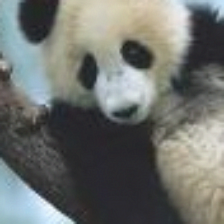
\includegraphics[width=.2\textwidth]{gibbon_993.png} \\
		$\centering \vec x$     &%
		& $\sgn \nabla_{\vec x} L(h(\vec x;\vec\theta), y)$ & & $\widetilde{\vec x}$ \\
		\emph{panda} (0.577) & & & & \emph{gibon} (0.993) 
	\end{tabular}
	\caption{Generiranje neprijateljskog primjera jednim korakom u smjeru predznaka gradijenta gubitka s obzirom na ulaz. Nakošene riječi predstavljaju razrede, a brojevi u zagradama vjerojatnosti koje neuronska mreža dodjeljuje razredima.}
	\label{panda}
\end{figure}	
\end{itemize}
\end{frame}
\note[itemize]{}

\begin{frame}{Pronalaženje neprijateljskih primjera}
	\begin{itemize}
		\item Neka $ B_\epsilon(\vec x)$ označava skup primjera takvih da je njihova udaljenost od prirodnog primjera $\vec x$ manja od $\epsilon$. 
		\item Neprijateljski primjeri se mogu pronaći rješavanjem optimizacijskog problema s ograničenjem:
		\begin{equation}
		\widetilde{\vec x} = \argmax_{\widetilde{\vec x}\in B_\epsilon(\vec x)} L(h(\widetilde{\vec x};\vec \theta), y).
		\end{equation}
		\item Ako su poznati parametri mreže koju se napada, neprijateljske primjere moguće je pronaći postupcima koji se temelje na gradijentnom spustu.
		\item Mogući su i napadi bez uvida u strukturu modela, npr. genetskim algoritmom.
		\item Također, pokazalo se da su neprijateljski primjeri u velikoj mjeri prenosivi između različitih modela.
	\end{itemize}
\end{frame}

\begin{frame}{Pronalaženje neprijateljskih primjera}
\begin{itemize}
	\item Već je jednim pomakom u smjeru predznaka gradijenta moguće pronalaziti neprijateljske primjere (\emph{fast gradient sign method}, FGSM):
	\begin{equation}
\widetilde{\vec x} = \vec x + \epsilon\sgn \nabla_{\vec x} L(h(\vec x;\vec\theta), y).
	\end{equation}
	\item Jači su iterativni postupci kao što je PGD (\emph{projected gradient descent}):
	\begin{equation} \label{eq:pgd}
\widetilde{\vec x} \gets \Pi_{B_\epsilon(\vec x)} (\widetilde{\vec x} + \alpha\sgn\nabla_{\widetilde{\vec x}} L(h(\widetilde{\vec x};\vec\theta), y)),
	\end{equation}
	gdje je $\Pi_{B_\epsilon(\vec x)}$ projekcija na susjedstvo od $\vec x$, $\Pi_{B_\epsilon(\vec x)}(\vec v) = \argmin_{\vec v'\in B_\epsilon(\vec x)}\lVert \vec v'-\vec v\rVert_\infty$.
\end{itemize}
\end{frame}

\begin{frame}{Neprijateljski rizik}
\begin{itemize}
	\item Može se definirati oblik rizika koji se može nazvati \emph{neprijateljskim rizikom}:
	\begin{equation}\label{eq:adv-risk}
\widetilde{R}(\vec\theta) = \widetilde{R}(\vec\theta;d,\epsilon) = \mathbb{E}_{(\vec x,y)\sim\mathcal{D}}\left[
\max_{\widetilde{\vec x} \in B_\epsilon(\vec x)} L(h(\widetilde{\vec x};\vec\theta), y) \right].
	\end{equation}
	\item Mali neprijateljski rizik predstavlja dobru lokalnu generalizaciju u susjedstvu prirodnih primjera.
\end{itemize}
\end{frame}

\begin{frame}{Učenje s neprijateljskim primjerima}
\begin{itemize}
	\item Trenutno najuspješniji pristup za postizanje otpornosti na neprijateljske primjere je učenje s neprijateljskim primjerima (engl. \emph{adversarial training}) dobivenim PGD-om.
	\item Kod učenja s neprijateljskim primjerima skup za učenje se proširuje neprijateljskim primjerima koji se tijekom učenja prilagođavaju parametrima mreže.
\end{itemize}
\end{frame}

\begin{frame}{Parsevalove mreže}
\begin{itemize}
	\item Kod Parsevalovih mreža se kontrolira Lipschitzova konstanta svih slojeva i cijele mreže tako da ne bude veća od $1$.
	\item Lipschitzova konstanta funkcije $f$, ako postoji, definirana je ovako:
	\begin{equation}
	\Lambda = \sup_{\vec x\neq \widetilde{\vec x}} \frac{\lVert f(\vec x)-f(\widetilde{\vec x})\rVert}{\lVert \vec x-\widetilde{\vec x}\rVert}.
	\end{equation}
	
	\item Važno svojstvo Parsevalovih mreža je da su matrice težina ortogonalne (poopćeno na nekvadratne matrice). Kod konvolucijskih mreža to znači da su konvolucijski filtri istog sloja međusobno ortogonalni.
	\item Prema autorima, takve mreže postižu bolju otpornost na neprijateljske primjere generirane FGSM-om od odgovarajućih mreža koje nisu Parsevalove, brže se uče i njihov kapacitet se bolje iskorištava.
\end{itemize}
\end{frame}

\begin{frame}{Ograničavanje neprijateljskog rizika Lipschitzovom konstantom}
\begin{itemize}
	\item Neuronska mreža se može prikazati kao usmjereni aciklički računski graf $G = (\mathcal{N}, \mathcal{E})$ gdje je svaki čvor $n\in\mathcal{N}$ funkcija svoje djece:
	\begin{equation}
	n(\vec x)=f^{(n)}(\vec\theta^{(n)}, (n'(\vec x))_{n':(n,n')\in\mathcal{E}}).
	\end{equation}
	\item Funkcija $h(\vec x) = h(\vec x;\vec\theta)$ koju ostvaruje mreža je korijen toga grafa. 
	\item U nastavku će $n'\lessdot n$ označavati da je $n$ roditelj od $n'$, tj. $(n,n')\in\mathcal{E}$.
\end{itemize}
\end{frame}

\begin{frame}{Ograničavanje neprijateljskog rizika Lipschitzovom konstantom}
\begin{itemize}
	\item Neka je $g(\vec x)$ funkcija koju predstavlja sloj logita s obzirom na ulaz mreže (izlaz je $h(\vec x)=\softmax(g(\vec x))$).
	\item Gubitak unakrsne entropije je $L(h(\vec x;\vec\theta), y) = -\ln h(\vec x;\vec\theta)_y$.
	\item Gubitak izražen preko $g$: $\ell(g(\vec x;\vec\theta),y) := L(h(\vec x;\vec\theta), y) = -g(\vec x;\vec\theta)_y + \ln \sum_{y'\in\mathcal{Y}}\exp(g(\vec x)_{y'}).$
	\item Neka za zadanu $p$-normu postoji $\lambda_p$ takav da
	\begin{equation} \label{eq:loss-lipschitz}
	\forall z,z'\in \mathbb{R}^C, \forall y\in\mathcal{Y},
	\lvert \ell(z,y)-\ell(z',y)\rvert 
	\leq \lambda_p\lVert z-z'\rVert_p.
	\end{equation}
	Najmanji takav $\lambda_p$ je Lipschitzova konstanta gubitka s obzirom na logite, npr. $\lambda_\infty=2$ i $\lambda_2=\sqrt2$.
\end{itemize}
\end{frame}

\begin{frame}{Ograničavanje neprijateljskog rizika Lipschitzovom konstantom}
\begin{itemize}
	\item Za svaki $p$ i $\epsilon > 0$  iz izraza~\ref{eq:loss-lipschitz} i definicije rizika $R(\vec\theta)$ i neprijateljskog rizika $\widetilde{R}(\vec\theta)=\widetilde{R}(\vec\theta,p,\epsilon)$ može se pokazati da vrijedi
	\begin{align}
	\widetilde{R}(\vec\theta) 
	&\leq R(\vec\theta) + \mathbb{E}_{(\vec x,y)\sim\mathcal{D}}\left[
	\max_{\widetilde{\vec x} \in B_\epsilon(\vec x)} \lvert \ell(g(\vec x;\vec\theta),y)-\ell(g(\vec x;\vec\theta),y) \rvert \right] \\
	&\leq R(\vec\theta) + \lambda_p\Lambda_p\epsilon.
	\end{align}
	\item Budući da uvijek vrijedi $R(\vec\theta) \leq \widetilde{R}(\vec\theta)$, slijedi da se smanjivanjem Lipschitzove konstante smanjuje razlika između $\widetilde{R}(\vec\theta)$ i $R(\vec\theta)$:
	\begin{equation}
	0 \leq \widetilde{R}(\vec\theta)-R(\vec\theta) \leq \lambda_p\Lambda_p\epsilon.
	\end{equation}
	\item Smanjivanje Lipschitzove konstante samo po sebi ne mora poboljšati otpornost na neprijateljske primjere. Npr. skaliranje logita nekom malom konstantom prije $\softmax$-a smanjuje $\widetilde{R}(\vec\theta)-R(\vec\theta)$, ali ne utječe na klasifikaciju.
\end{itemize}
\end{frame}

\begin{frame}{Lipschitzova konstanta neuronske mreže}
\begin{itemize}
	\item Neka $\Lambda_p^{(n)}$ označava Lipschitzovu kostantu čvora $n$ s obzirom na ulaz mreže, a $\Lambda_p^{(n,n')}$ Lipschitzovu konstantu čvora $n$ s obzirom na njemu ulazni čvor $n'$. Vrijedi
	\begin{equation}
	\Lambda_p^{(n)} = \sum_{n'\lessdot n}
	\Lambda_p^{(n,n')}\Lambda_p^{(n')}.
	\end{equation}
	
	\item Za sloj linearnog preslikavanja vrijedi: 
	\begin{align}
	n(\vec x) &= \mat W^{(n)}n'(\vec x) \\
	\Lambda_p^{(n)} &\leq \lVert \mat W^{(n)}\rVert_p\Lambda_p^{(n')}.
	\end{align}
\end{itemize}
\end{frame}

\begin{frame}{Lipschitzova konstanta neuronske mreže}
\begin{itemize}
	\item Kod konvolucijskog sloja kod kojega konvoluciji s $r$-tom jezgrom odgovara izraz $n(\vec x)^{(r)} = \tens w^{(n,r)}*_d n'(\vec x)$ računanje izlaza može se prikazati kao matrično množenje $\mat W^{(n)}U(n'(\vec x))$., gdje je $\mat W$ matrica kojoj su reci filtri izravnati u vektore, a $U$ operator koji ulaz pretvara u matricu kod koje svaki stupac sadrži elemente ulaza koji su za pojedini prostorni položaj ulaza prekriveni konvolucijskom jezgrom. Može se pokazati da vrijedi
	\begin{align} \label{eq:konv-lipschitz}
	\Lambda_2^{(n)} &\leq \sqrt{K} \lVert \mat W^{(n)}\rVert_2\Lambda_2^{(n')}, \\ \Lambda_\infty^{(n)} &\leq \lVert \mat W^{(n)}\rVert_\infty\Lambda_\infty^{(n')},
	\end{align}
	gdje je $K$ broj elemenata jezgre podijeljen sa semantičkom dimenzijom ulaza. 
\end{itemize}
\end{frame}

\begin{frame}{Lipschitzova konstanta neuronske mreže}
\begin{itemize}
	\item Kod aktivacijskih slojeva Lipschitzova konstanta s obzirom na ulaz čvora odgovara Lipschitzovoj konstanti prijenosne funkcije $\lambda_p^{(n)}$ pa vrijedi:
	\begin{equation}
	\Lambda_p^{(n)} \leq \lambda_p^{(n)}\Lambda_p^{(n')}.
	\end{equation}
		
	\item Kod slojeva linearne kombinacije vrijedi $n(\vec x) = \sum_{n'\lessdot n}\alpha^{(n,n')}n'(\vec x)$, gdje su $\alpha^{(n,n')}$ skalari. Za Lipschitzovu konstantu vrijedi
	\begin{equation} \label{eq:linear-combination}
	\Lambda_p^{(n)} \leq \sum_{n'\lessdot n}\alpha^{(n,n')}\Lambda_p^{(n')}.
	\end{equation}
	\item Poseban slučaj takvog čvora je čvor zbrajanja kod preskočnih veza u rezidualnim mrežama. Za takav čvor je
	\begin{equation}
	\Lambda_p^{(n)} \leq \sum_{n'\lessdot n}\Lambda_p^{(n')}.
	\end{equation}
\end{itemize}
\end{frame}

\begin{frame}{Parsevalove mreže: ortogonalnost matrica težina}
\begin{itemize}
	\item Kako bi se osiguralo ograničenje Lipschitzove konstante kroz cijelu mrežu, autori predlažu održavanje redaka matrica težina ortonormiranima i zamjenu zbrojeva kod preskočnih veza konveksnim kombinacijama.
	\item Kako bi se reci matrica težina održali ortogonalnima, nakon svakog koraka učenja ažuriraju se težine jednim korakom gradijentnog spusta s obzirom na gubitak $R_\beta(\mat W) = \frac{\beta}{2}\lVert \mat W \mat W^\transpose-\mat I\rVert_2^2$:
	\begin{equation}
	\mat W \gets (1+\beta)\mat W-\beta \mat W\mat W^\transpose \mat W. 
	\end{equation}
\end{itemize}
\end{frame}

\begin{frame}{Parsevalove mreže: konveksne kombinacije}
\begin{itemize}
	\item U Parsevalovim mrežama se čvorovi zbrajanja zamjenjuju čvorovima konveksne kombinacije čije se težine uče.
	\item  U slučaju preskočnih veza zbroj se zamjenjuje konveksnom kombinacijom
	$n(\vec x) = \alpha n'(\vec x) + (1-\alpha)n''(\vec x)$, gdje su $n'$ i $n''$ djeca čvora $n$. Parametar $\alpha$ se uči gradijentnim spustom i  ograničavanje koeficijenta je onda jednostavno: $\alpha\gets\min\{\max\{\alpha, 0\},1\}$.
\end{itemize}
\end{frame}

\begin{frame}{Rezultati autora}
\begin{itemize}
	\item Autori zaključuju da se kod Parsevalovih mreža poboljšava otpornost na neprijateljske primjere, ubrzava učenje i bolje iskorištva kapacitet mreže.
	\item Dalje će biti prikazani rezultati koje su autori dobili za rezidualnu mrežu WRN-28-10 i odgovarajuću Parsevalovu mrežu uz korištenje FGSM-a za dobivanje neprijateljskih primjera.
\end{itemize}
\end{frame}

\begin{frame}{Rezultati autora}
\begin{table}[h!]
	\begin{center}
		\bgroup\footnotesize
		\begin{tabular}{|c|l|c|c|c|c|c|}
			\hline
			{\bf }
			& {\bf Model}
			& {\bf Bez šuma} & {\bf $\varepsilon\approx50$} & {\bf $\varepsilon\approx45$} & {\bf $\varepsilon\approx40$} & {\bf $\varepsilon\approx33$} \\
			\hline
			\multirow{6}{*}{\rotatebox{90}{CIFAR-10}}
			& Vanilla
			& 95.63         & 90.16         & 85.97         & 76.62         & 67.21      \\
			& Parseval(OC)
			& 95.82         & 91.85         & 88.56         & 78.79         & 61.38      \\
			& Parseval
			& \textbf{96.28}          & \textbf{93.03}         & \textbf{90.40}         & \textbf{81.76}         & \textbf{69.10}      \\
			\cline{2-7}
			\cline{2-7}
			& Vanilla
			& 95.49         & 91.17         & 88.90         & 86.75         & 84.87      \\
			& Parseval(OC)
			& 95.59         & 92.31         & 90.00         & \textbf{87.02}         & \textbf{85.23}      \\
			& Parseval
			& \textbf{96.08}          & \textbf{92.51}         & \textbf{90.05}         & 86.89         & 84.53      \\
			\hline\hline
			\multirow{6}{*}{\rotatebox{90}{CIFAR-100}}
			& Vanilla
			& 79.70         & 65.76         & 57.27         & 44.62         & 34.49      \\
			&Parseval(OC)
			& 81.07         & 70.33         & 63.78         & 49.97         & 32.99      \\
			& Parseval
			& \textbf{80.72}          & \textbf{72.43}         & \textbf{66.41}         & \textbf{55.41}         & \textbf{41.19}      \\
			\cline{2-7}
			\cline{2-7}
			& Vanilla
			& 79.23         & 67.06         & 62.53         & 56.71         & 51.78      \\
			& Parseval(OC)
			& \textbf{80.34}         & 69.27         & 62.93         & 53.21         & \textbf{52.60}      \\
			& Parseval
			& 80.19          & \textbf{73.41}         & \textbf{67.16}         & \textbf{58.86}         & 39.56      \\
			\hline
		\end{tabular}
		\egroup
	\end{center}
	\caption{
		Točnost klasifikacije mreže WRN-28-10 na skupovima CIFAR-10 i CIFAR-100. $\varepsilon$ je omjer signala i šuma dobivenog FGSM-om u decibelima. Za $\varepsilon=30$ čovjek može prepoznati da je dodan neprijateljski šum. Za svaki skup podataka prva 3 retka su rezultati za učenje bez neprijateljskih primjera, a donja 3 retka s neprijatljskim primjerima. \emph{Parseval(OC)} označava mrežu na kojoj se ne koriste konveksne kombinacije, nego samo ograničenja ortogonalnosti.
	}\label{tab:adv-robustness}
\end{table}
\end{frame}


\begin{frame}{Rezultati autora}
\begin{figure}[htbp]
	\centering
	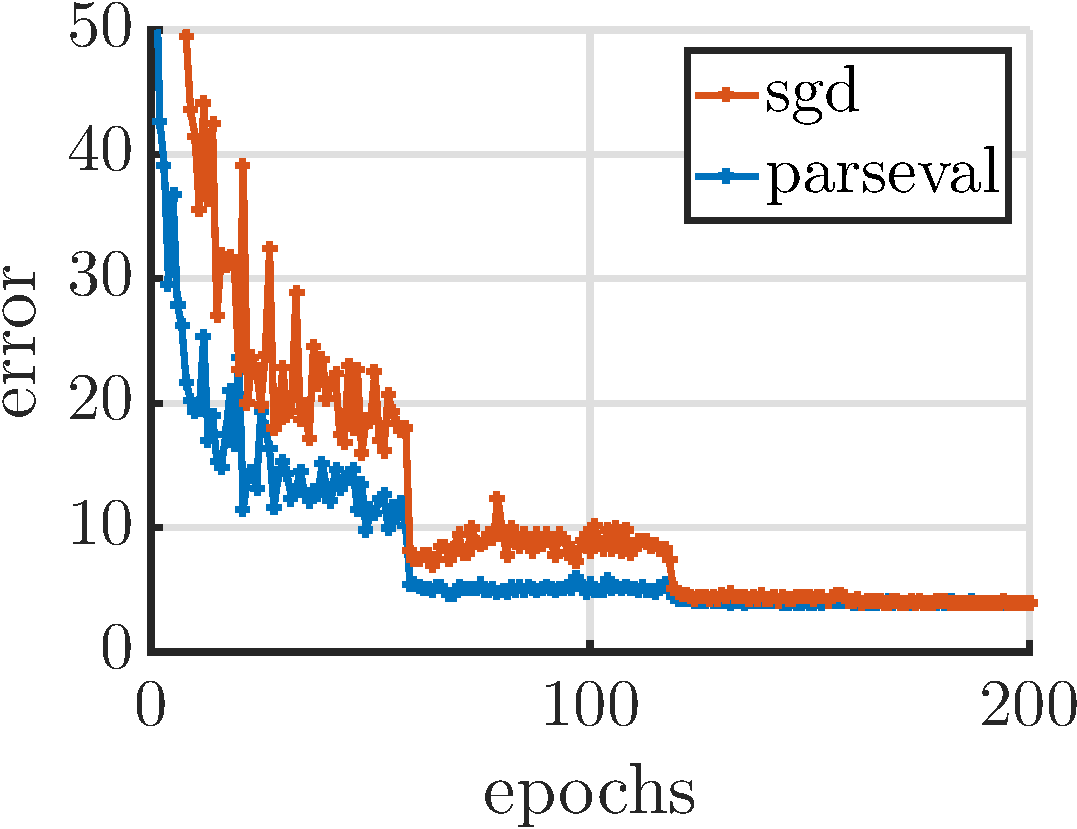
\includegraphics[width=0.49\linewidth]{ilustracije/convergence/cifar10.pdf}
	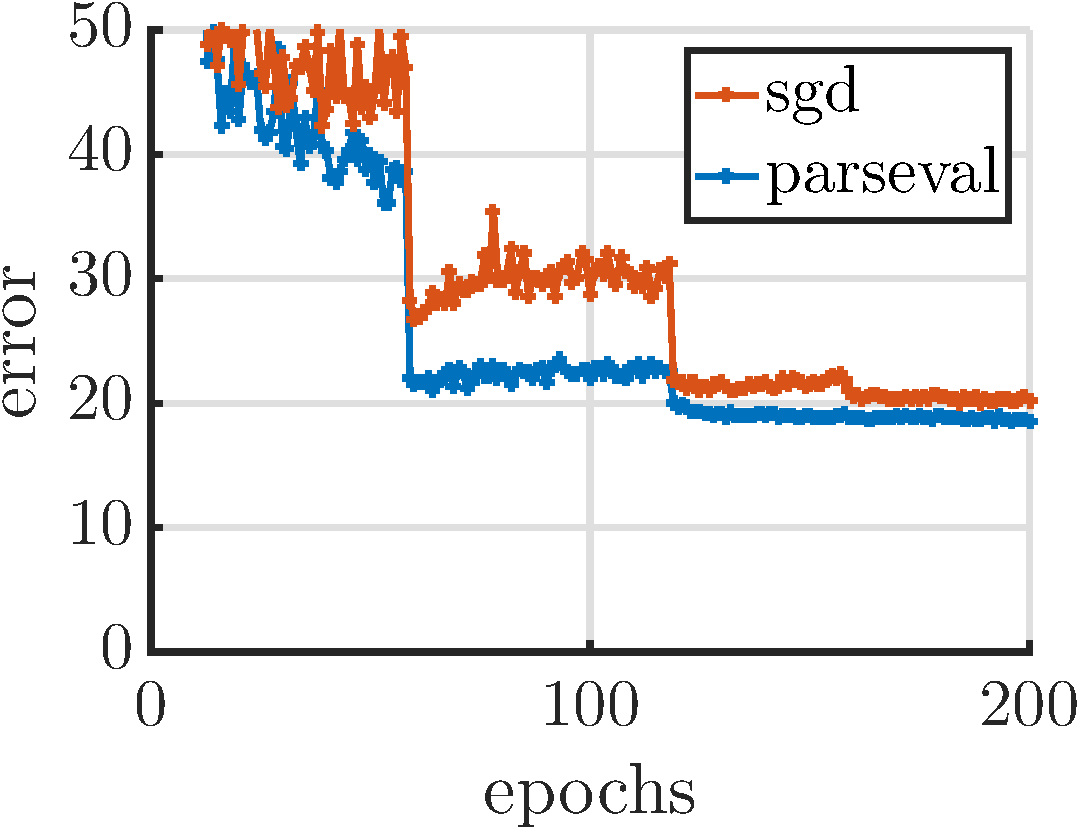
\includegraphics[width=0.49\linewidth]{ilustracije/convergence/cifar100.pdf}
	\caption{
		Krivulje koje pokazuju ovisnost klasifikacijske pogreške o broju završenih epoha koje su autori dobili učenjem obične (narančasto) i Parsevalove (plavo) mreže WRN-28-10 na skupovima CIFAR-10 (lijevo) i CIFAR-100 (desno). Slika je preuzeta iz članka.
	}
	\label{fig:krivulje-pogreske}
\end{figure}
\end{frame}

\begin{frame}{Zadatak projekta i rezultati}
\begin{itemize}
	\item Ostvarena je biblioteka za izgradnju rezidualnih mreža za Tensorflow.
	\item Ostvarene su rezidualna mreža WRN-28-10 i odgovarajuća Parsevalova mreža, ali zbog nečega postižu nižu klasifikacijsku točnost nego što bi trebale: oko $0.94$ umjesto $0.96$.
	\item Mreže su učene i testirane na skupu CIFAR-10.
\end{itemize}
\end{frame}

\begin{frame}{Zadatak projekta i rezultati}
\begin{figure}[htbp]
	\centering
	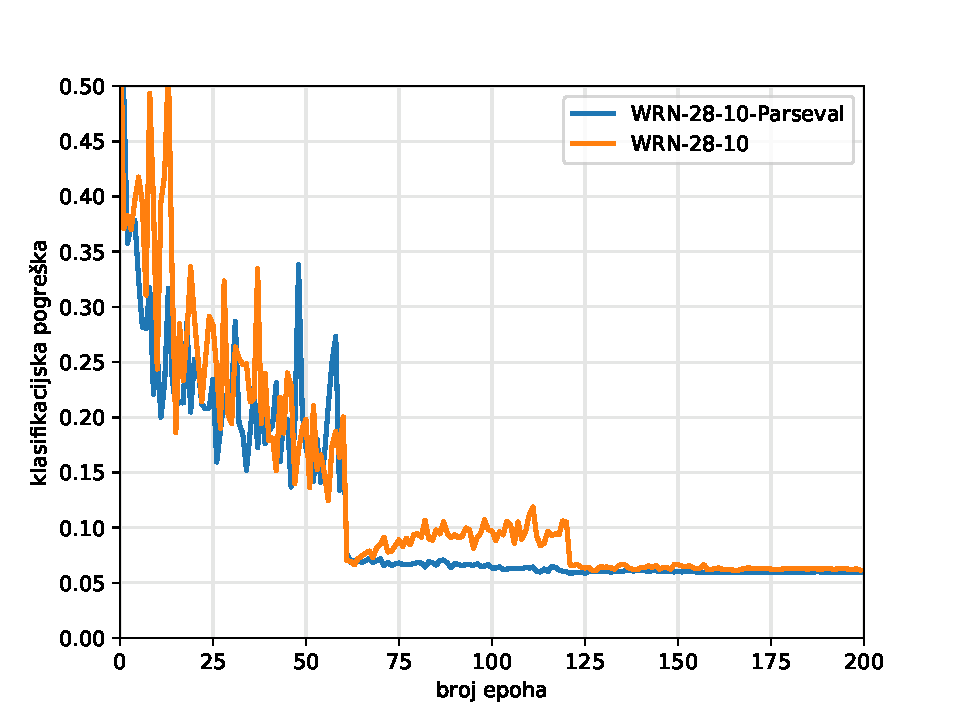
\includegraphics[width=0.65\linewidth]{ilustracije/grafovi/krivulje-pogreske}
	\caption{
		Ovisnost klasifikacijske pogreške o broju završenih epoha za Parsevalovu (plavo) i običnu (narančasto) rezidualnu mrežu. Svaka mreža se učila na uniji skupa za učenje i skupa za validaciju, a evaluirala na skupu za testiranje. Svaka krivulja je rezultat jednog mjerenja.
	}
	\label{fig:krivulje-pogreske-moje}
\end{figure}
\end{frame}

\begin{frame}{Zadatak projekta i rezultati}
\begin{figure}[htbp]
	\centering
	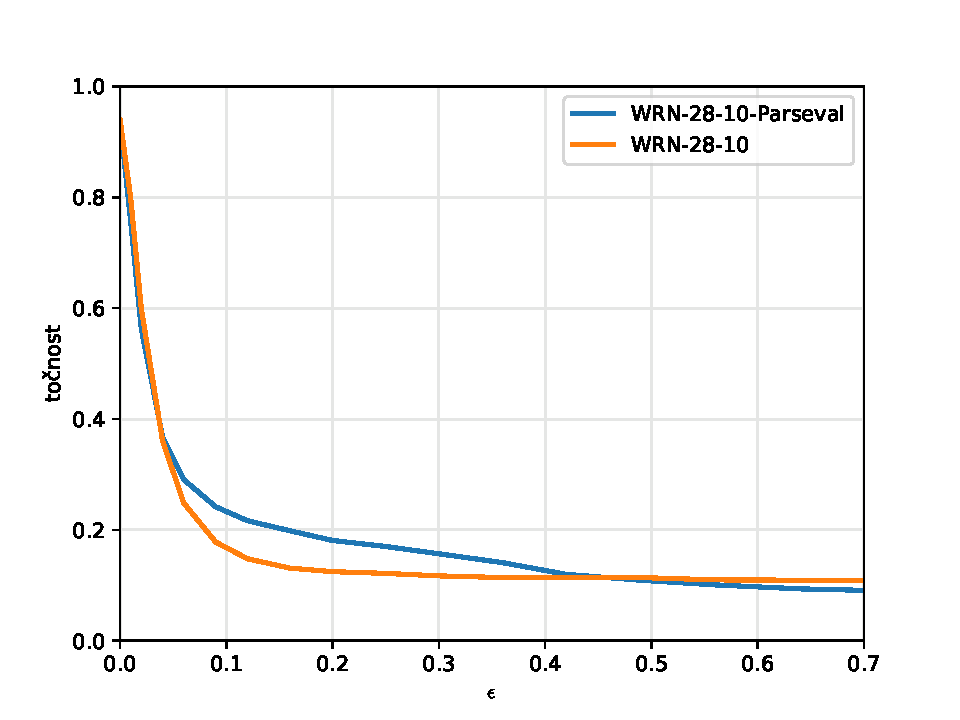
\includegraphics[width=0.65\linewidth]{ilustracije/grafovi/otpornost}
	\caption{
		Krivulje ovisnosti točnosti o iznosu $\infty$-norme šuma generiranog algoritmom FGSM za mreže iz slike~\ref{fig:krivulje-pogreske-moje}. Šum se dodaje normaliziranim slikama is podskupa za testiranje skupa CIFAR-10. Za dobivanje grafa su radi bržeg generiranja neprijateljskih primjera i evaluacije korištene 16384 slike iz skupa za testiranje.
	}
	\label{fig:krivulje-otpornosti}
\end{figure}
\end{frame}

\begin{frame}{Zadatak projekta i rezultati}
\begin{figure}[htbp]
	\centering
	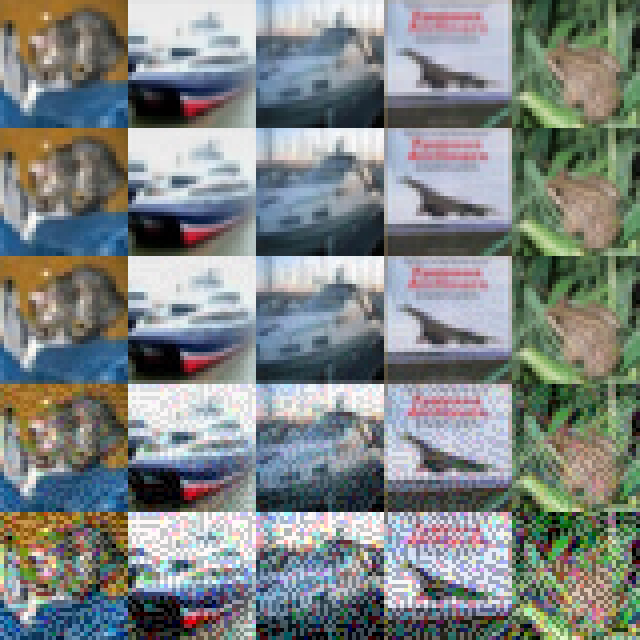
\includegraphics[width=0.55\linewidth]{ilustracije/slike/np-eps025251}
	\caption{
		Neprijateljski primjeri dobiveni FGSM-om za $\epsilon=0,0.02,0.05,0.2,0.5$ redom odozgo prema dolje.
	}
	\label{fig:neprijateljski-primjeri}
\end{figure}
\end{frame}

%\begin{frame}{Literatura}
%\bibliography{literatura}
\bibliographystyle{fer}

\nocite{colah}
\nocite{nndl}

%\end{frame}
\end{document}
